\documentclass[]{scrartcl}
\usepackage{amsmath}
\usepackage{graphicx}
\usepackage[hypcap]{caption}
\usepackage{geometry}
\usepackage{hyperref}
\geometry{
	a4paper,
	total={210mm,297mm},
	left=20mm,
	right=20mm,
	top=15mm,
	bottom=1mm,
}
 
 
% Title Page
\title{Theoretical part}
\author{Iliushin Vladislav}


\begin{document}
\maketitle

 
\section{}

\begin{equation} \label{eq:main_function}
   f(x) = f(c, r) 
\end{equation}

 \begin{itemize}
 	\item $ m $ is the number of points
 	\item $ \mathbf{x} = [x_1 \: y_1] $ is the center og the circle
 	\item $ r $ is  a circle radius
 	\item $ \mathbf{a_i} = [a_1 \: a_2 ] $ is a vector of the coordinates  $\mathbf{a_i} $
 	\item $ \mathbf{A} = [a_1 \dots a_i] $ is a vector of all given points
 \end{itemize}
 In our case  $ r = 1 $.  We will only change $ \mathbf{x} = [x_1 \: y_1] $ for given dataset $ \mathbf{A} = [a_1 \dots a_m] $.

\newpage
\subsection{}\label{section_1}
 \begin{itemize}
 	\item $m = 1$ 
 	\item $ \mathbf{A} = [0 \: 0] $
 	\begin{figure}[h]
 		\centering
 		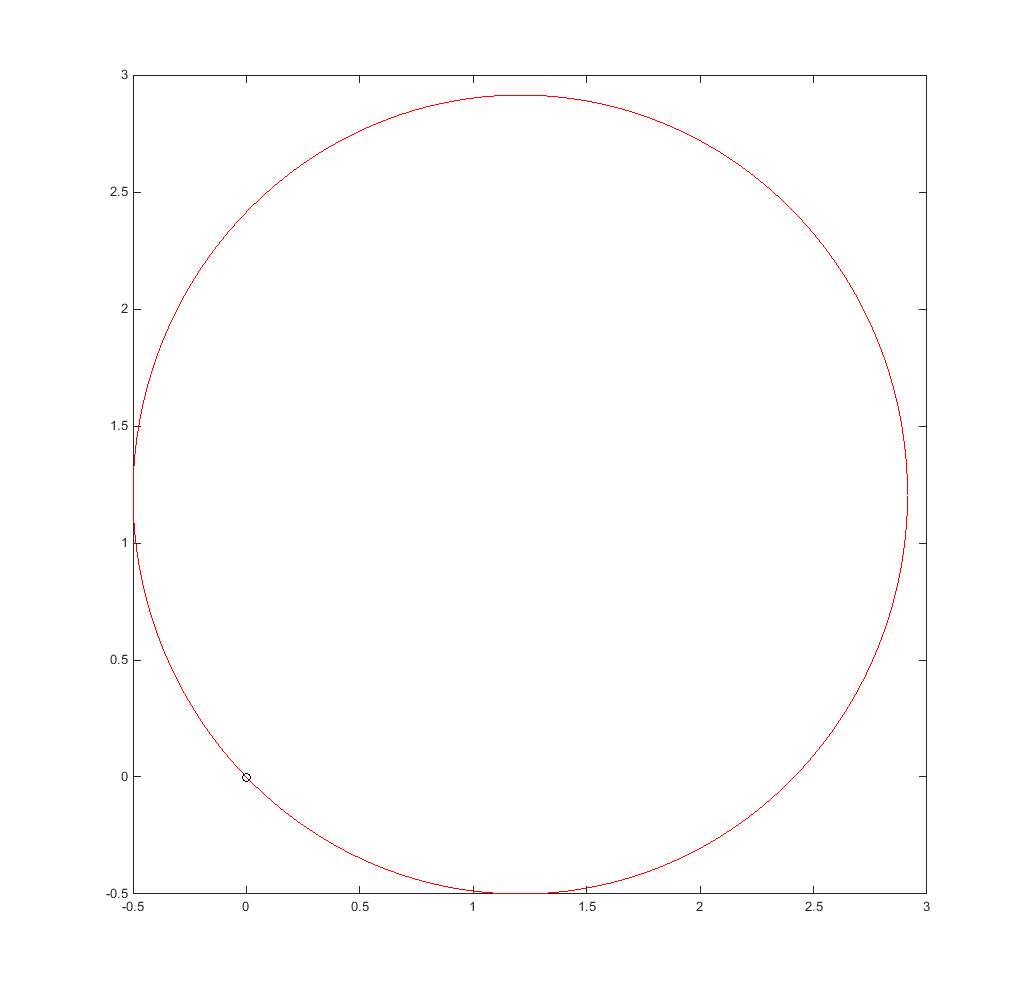
\includegraphics[width=0.5\textwidth]{1point_approx.eps}
 		\caption{Given points $\mathbf{ A} $ (black)}
 		\label{fig:m1gd}
 	\end{figure}
 \end{itemize}
\begin{figure}[h]
	\centering
	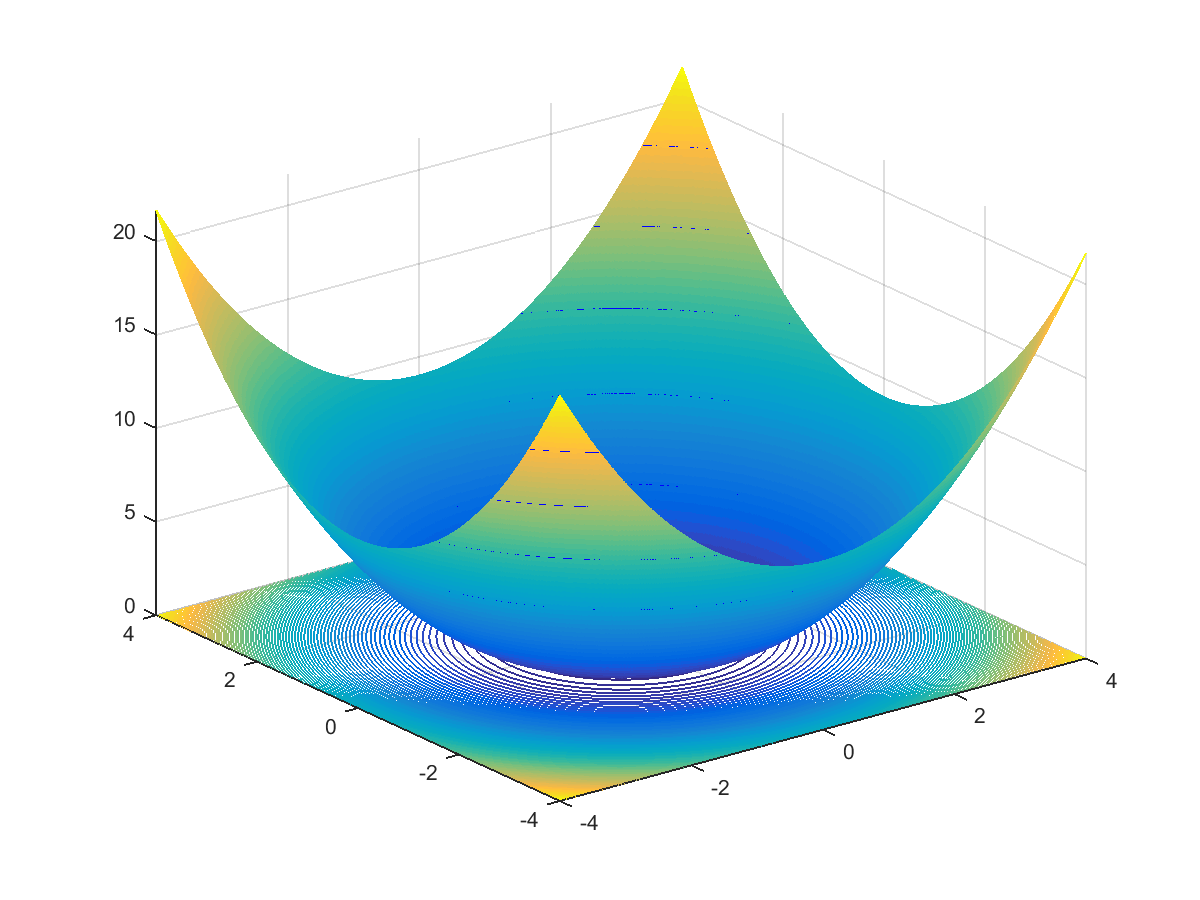
\includegraphics[width=0.5\textwidth]{1point_mesh.eps}
	\caption{Graph of the function ~\ref{eq:main_function} depending on the center of the circle}
	\label{fig:m13d}
\end{figure}
\begin{figure}[h]
	\centering
	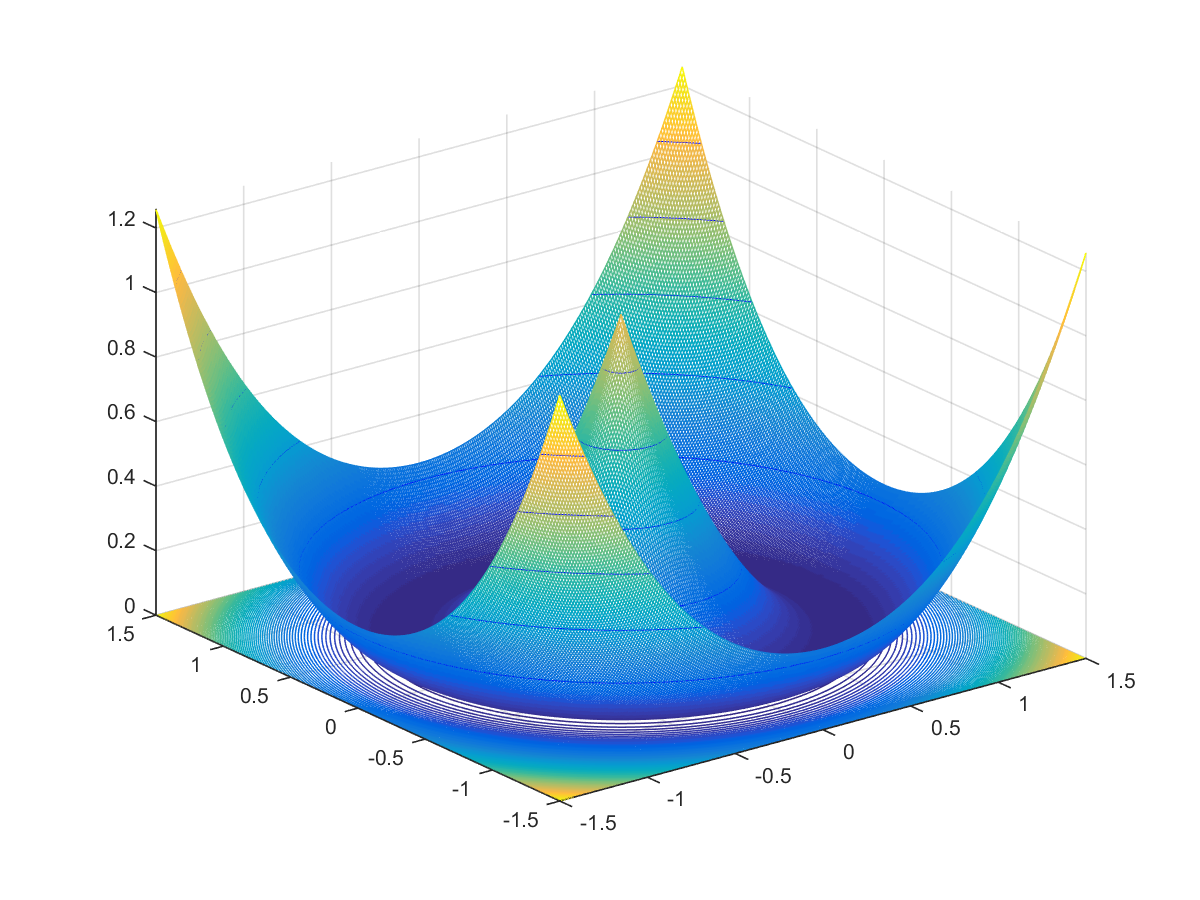
\includegraphics[width=0.5\textwidth]{1point_mesh_close.eps}
	\caption{Closer look at the graph of the function ~\ref{eq:main_function} depending on the center of the circle}
	\label{fig:m13dc}
\end{figure}
\begin{figure}[h]
	\centering
	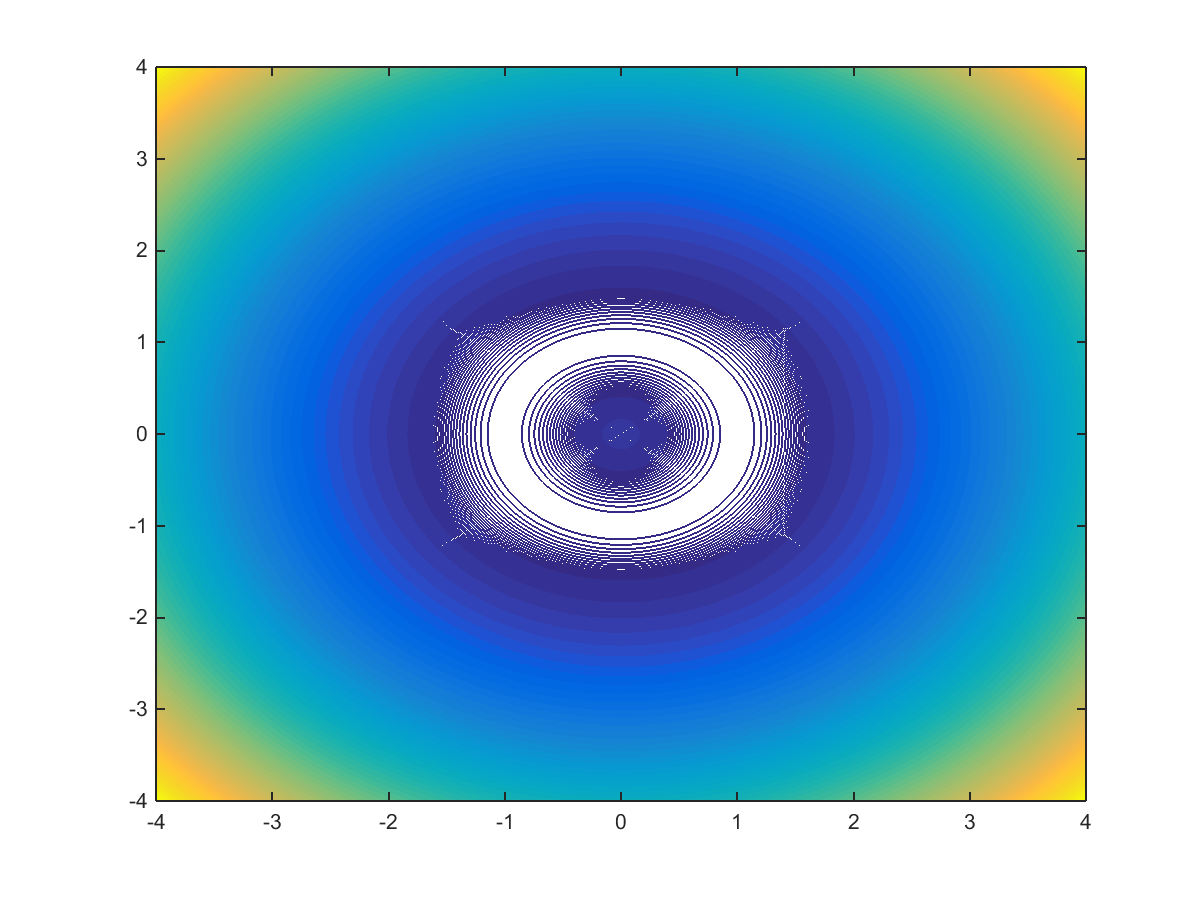
\includegraphics[width=0.5\textwidth]{1point_contour.png}
	\caption{Contour of the function ~\ref{eq:main_function} depending on the center of the circle}
	\label{fig:m12d}
\end{figure}
\begin{figure}[h]
	\centering
	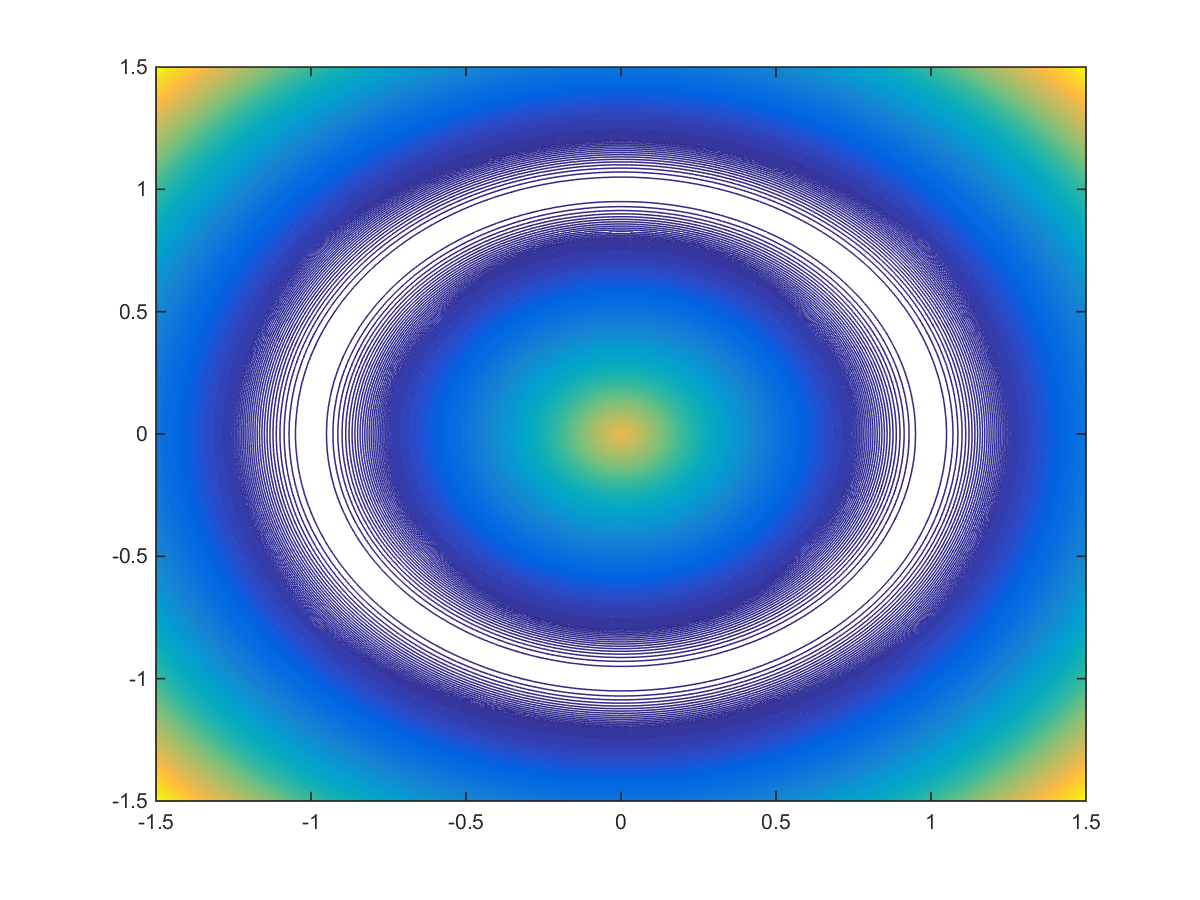
\includegraphics[width=0.5\textwidth]{1point_contour_close.png}
	\caption{Closer look at the contour of the function ~\ref{eq:main_function} depending on the center of the circle}
	\label{fig:m12dc}
\end{figure}


 \clearpage
\subsection{}\label{section_2}
 \begin{itemize}
 	\item $m = 2$ 
 	\item $ \mathbf{A} = [[-1 \: 0] \: [1 \: 0]] $
 	\begin{figure}[h]
 		\centering
 		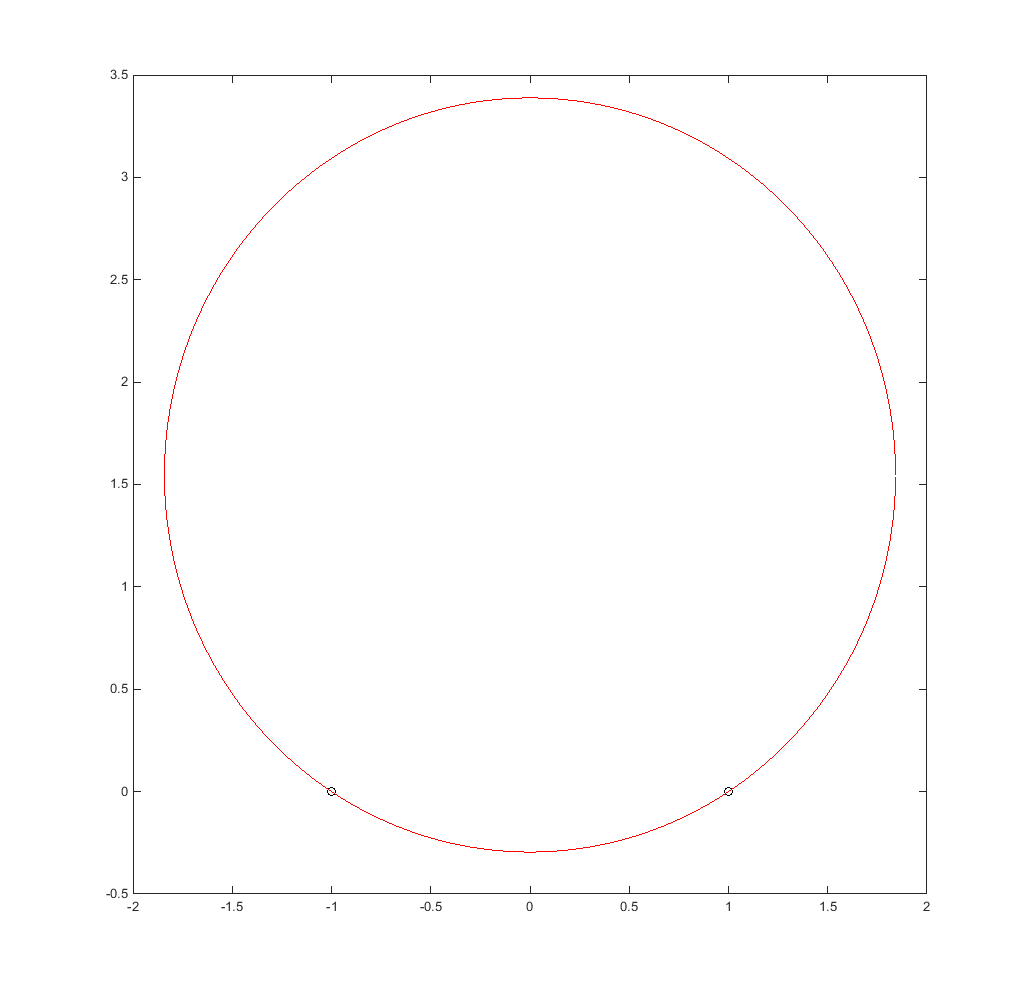
\includegraphics[width=0.5\textwidth]{2point_approx.eps}
 		\caption{Given points $\mathbf{ A} $ (black)}
 		\label{fig:m2gd}
 	\end{figure}
 \end{itemize}
 \begin{figure}[h]
 	\centering
 	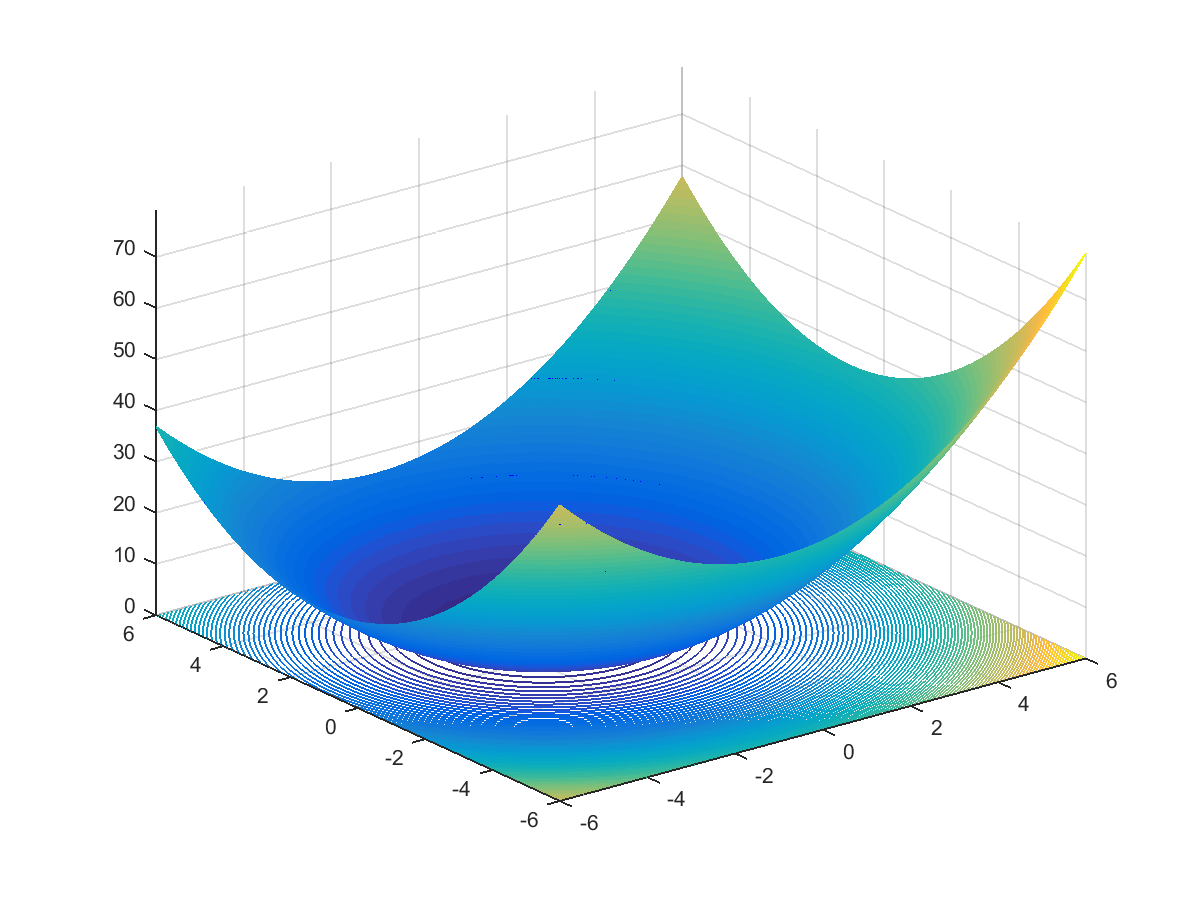
\includegraphics[width=0.5\textwidth]{2point_mesh.eps}
 	\caption{Graph of the function ~\ref{eq:main_function} depending on the center of the circle}
 	\label{fig:m23d}
 \end{figure}
 \begin{figure}[h]
 	\centering
 	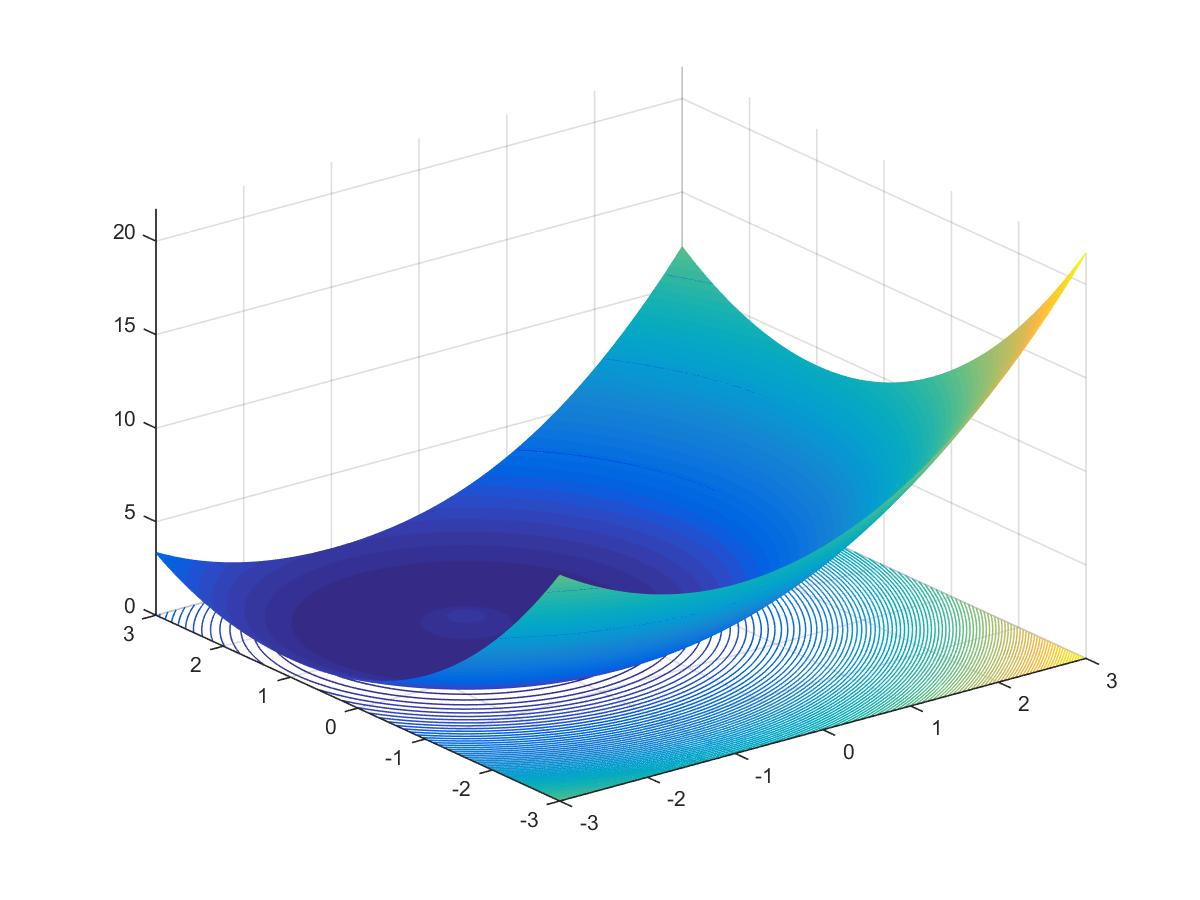
\includegraphics[width=0.5\textwidth]{2point_mesh_close.eps}
 	\caption{Closer look at the graph of the function ~\ref{eq:main_function} depending on the center of the circle}
 	\label{fig:m23dc}
 \end{figure}
 \begin{figure}[h]
 	\centering
 	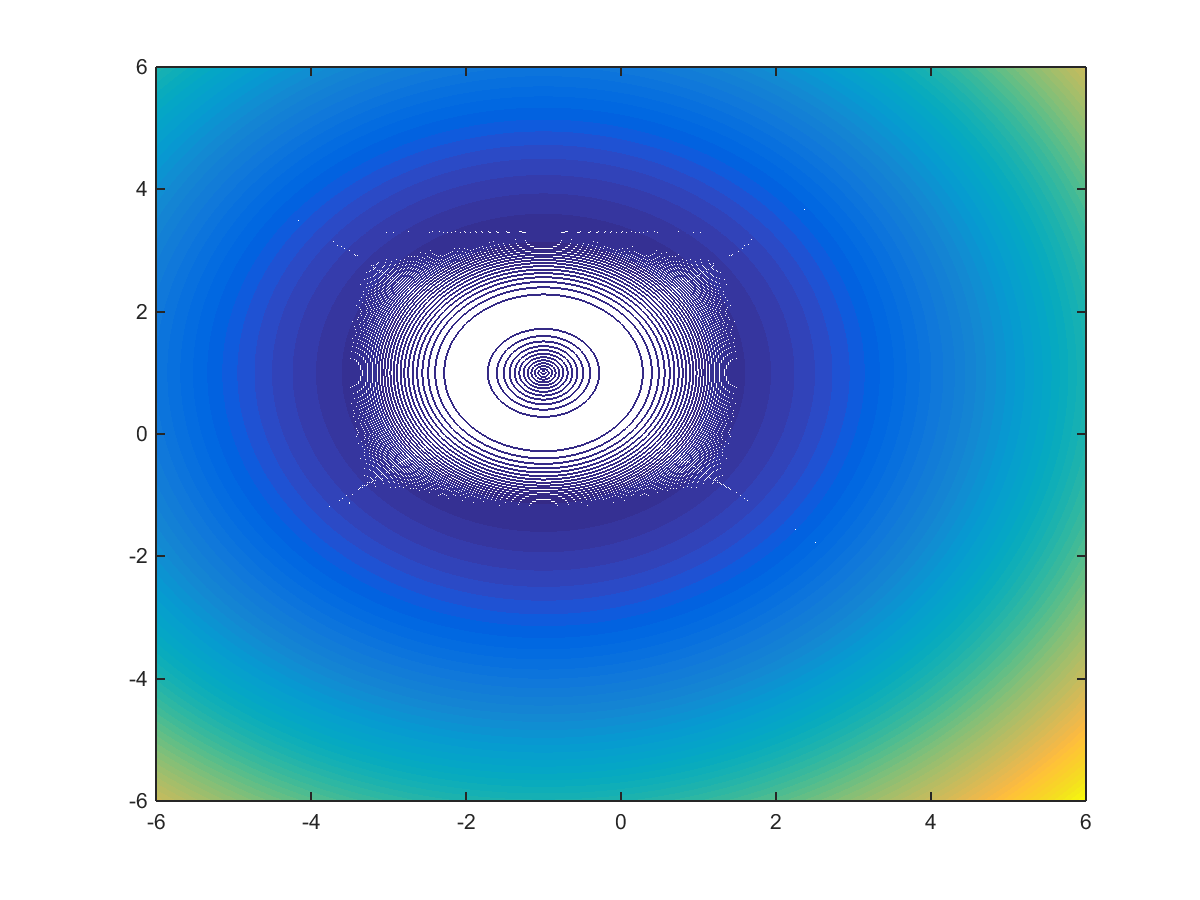
\includegraphics[width=0.5\textwidth]{2point_contour.png}
 	\caption{Contour of the function ~\ref{eq:main_function} depending on the center of the circle}
 	\label{fig:m22d}
 \end{figure}
  \begin{figure}[h]
  	\centering
  	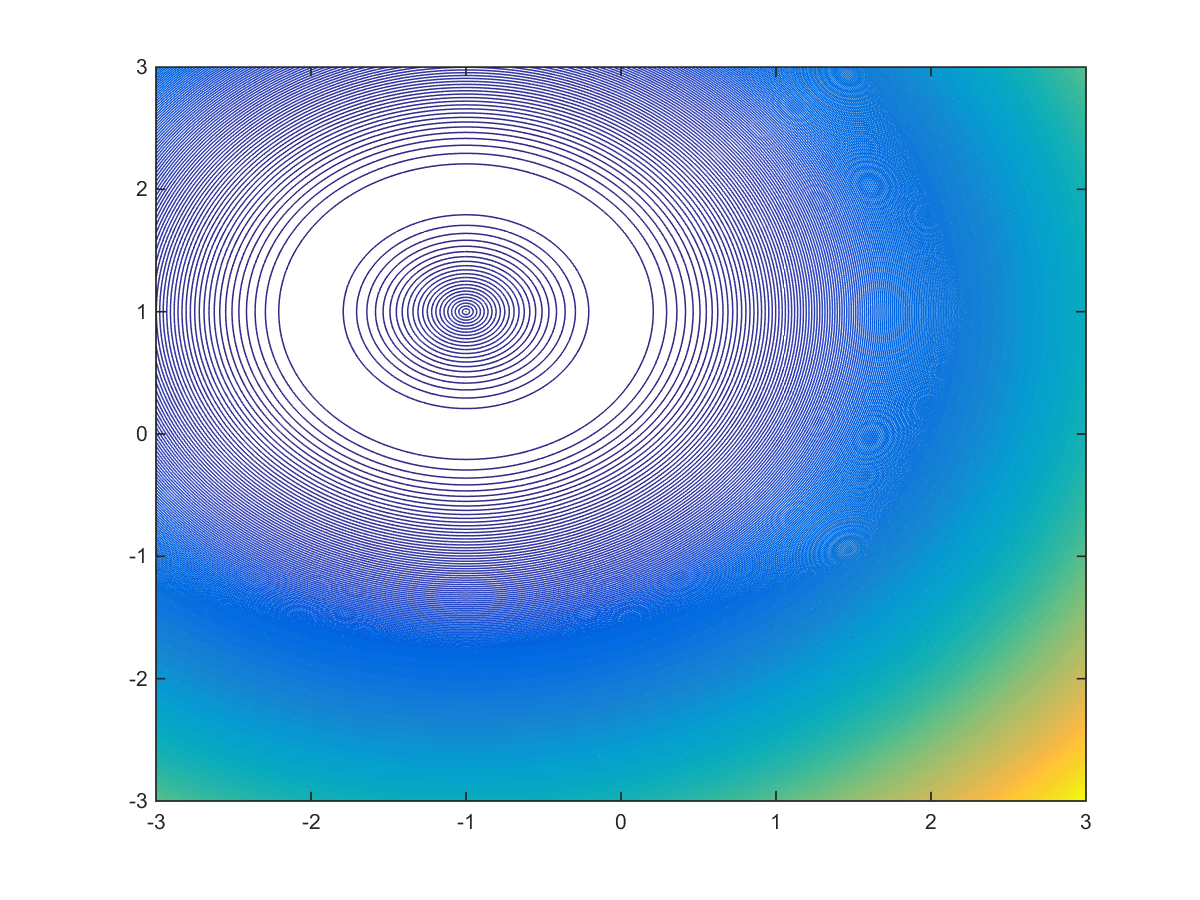
\includegraphics[width=0.5\textwidth]{2point_contour_close.eps}
  	\caption{Closer look at the contour of the function ~\ref{eq:main_function} depending on the center of the circle}
  	\label{fig:m22dc}
  \end{figure}
  
 
 \clearpage
 \subsection{}
 \begin{itemize}
 	\item $m = 9688$ 
 	\item $\mathbf{A }$ is a set of points  $\sin(x^2 + y^2) = \cos(xy)$
 	  \begin{figure}[h]
 		\centering
 		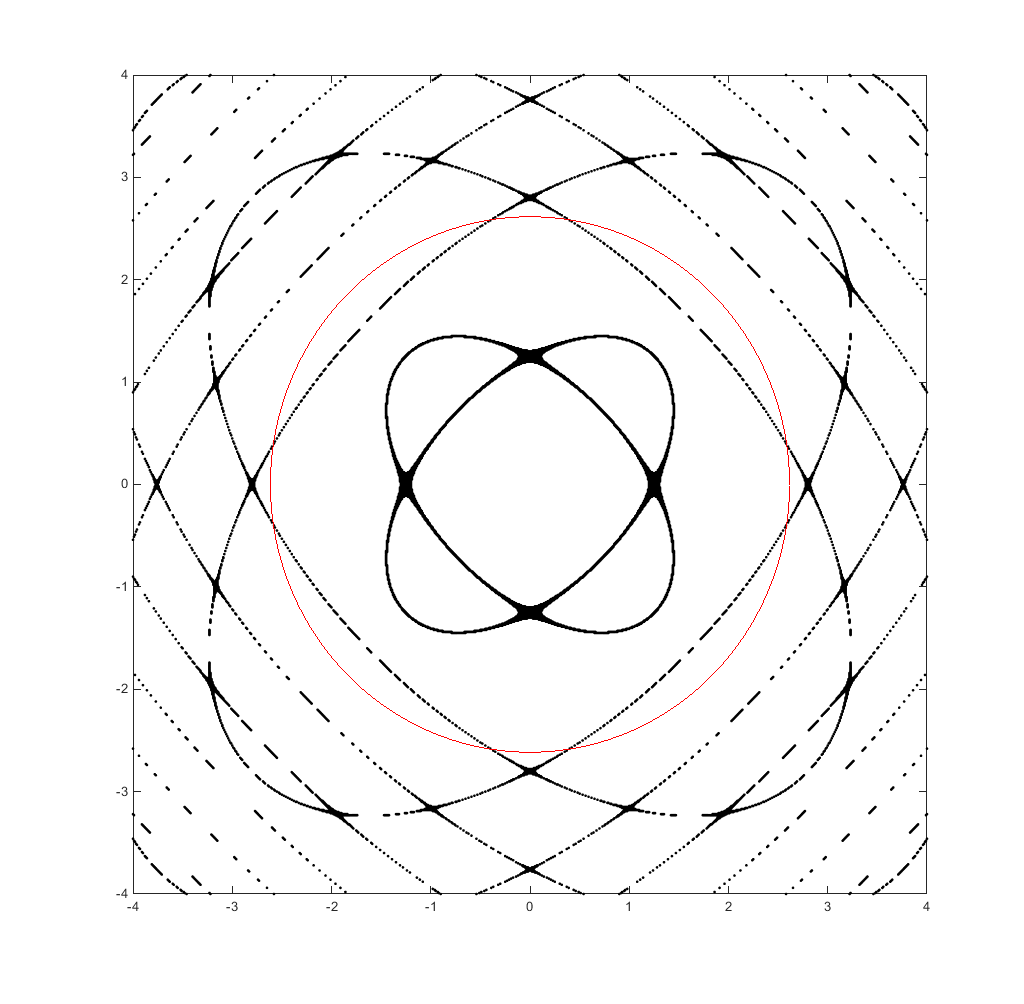
\includegraphics[width=0.5\textwidth]{9688point_approx.eps}
 		\caption{Given points $\mathbf{ A} $ (black)}
 		\label{fig:m9688gd}
 	\end{figure}
 \end{itemize}
 \begin{figure}[h]
 	\centering
 	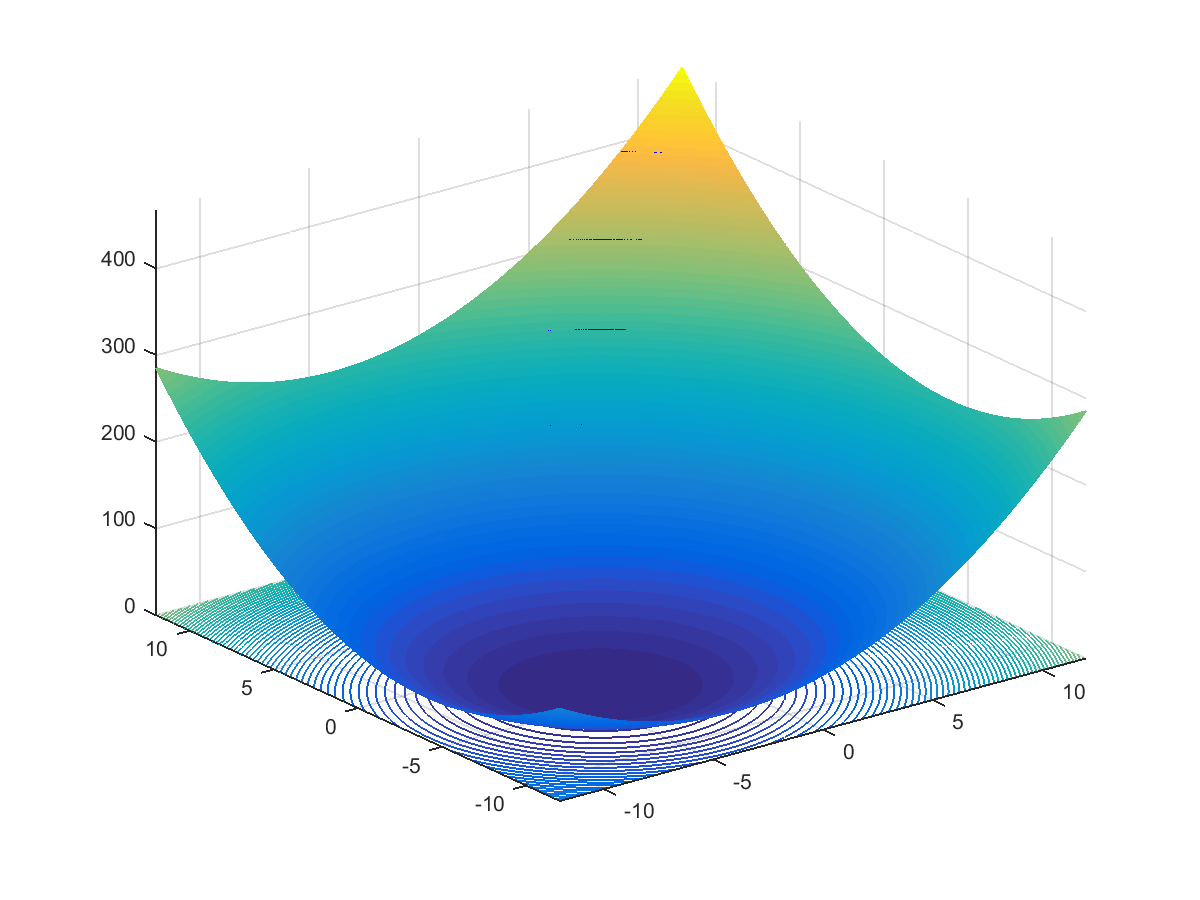
\includegraphics[width=0.5\textwidth]{9688point_mesh.eps}
 	\caption{Graph of the function ~\ref{eq:main_function} depending on the center of the circle}
 	\label{fig:m96883d}
 \end{figure}
  \begin{figure}[h]
  	\centering
  	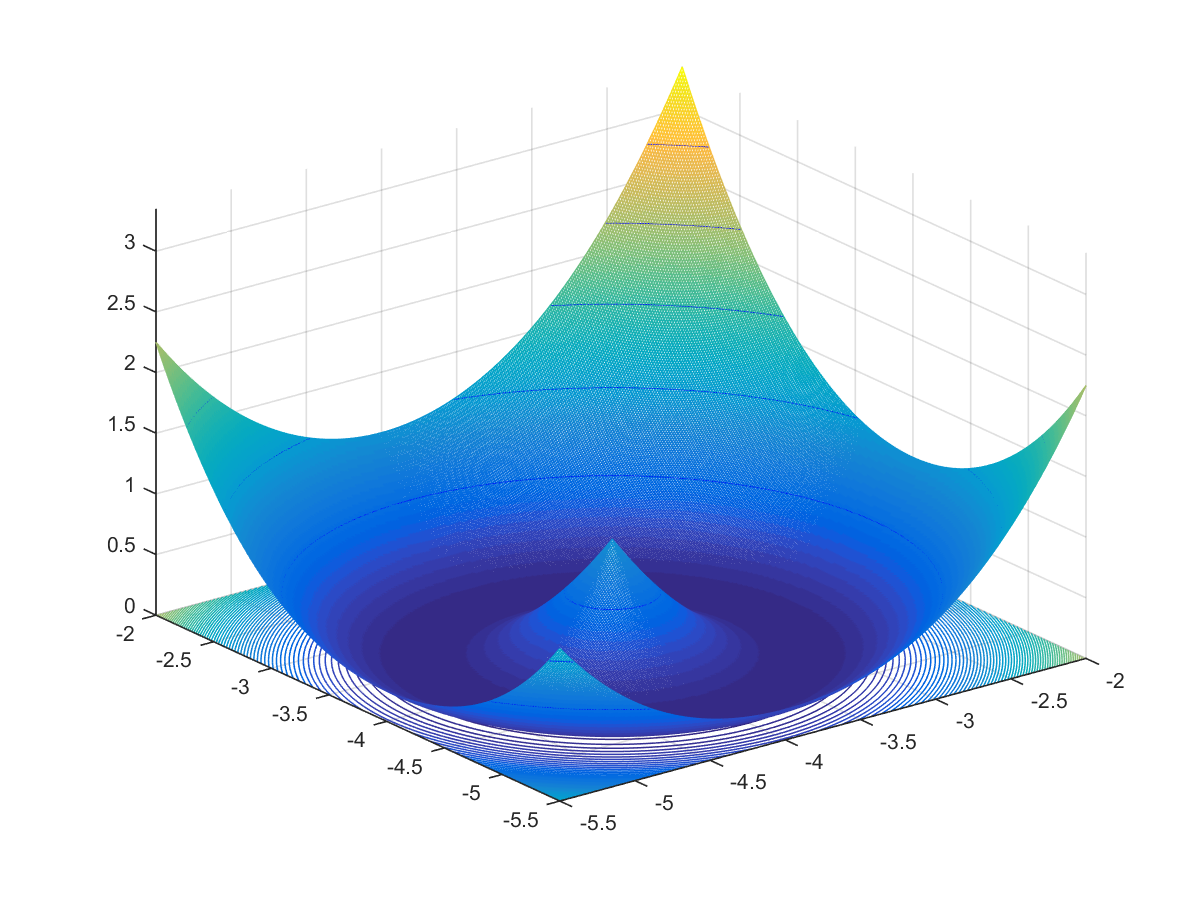
\includegraphics[width=0.5\textwidth]{9688point_mesh_close.eps}
  	\caption{Closer look at the graph of the function ~\ref{eq:main_function} depending on the center of the circle}
  	\label{fig:m96883dc}
  \end{figure}
 \begin{figure}[h]
 	\centering
 	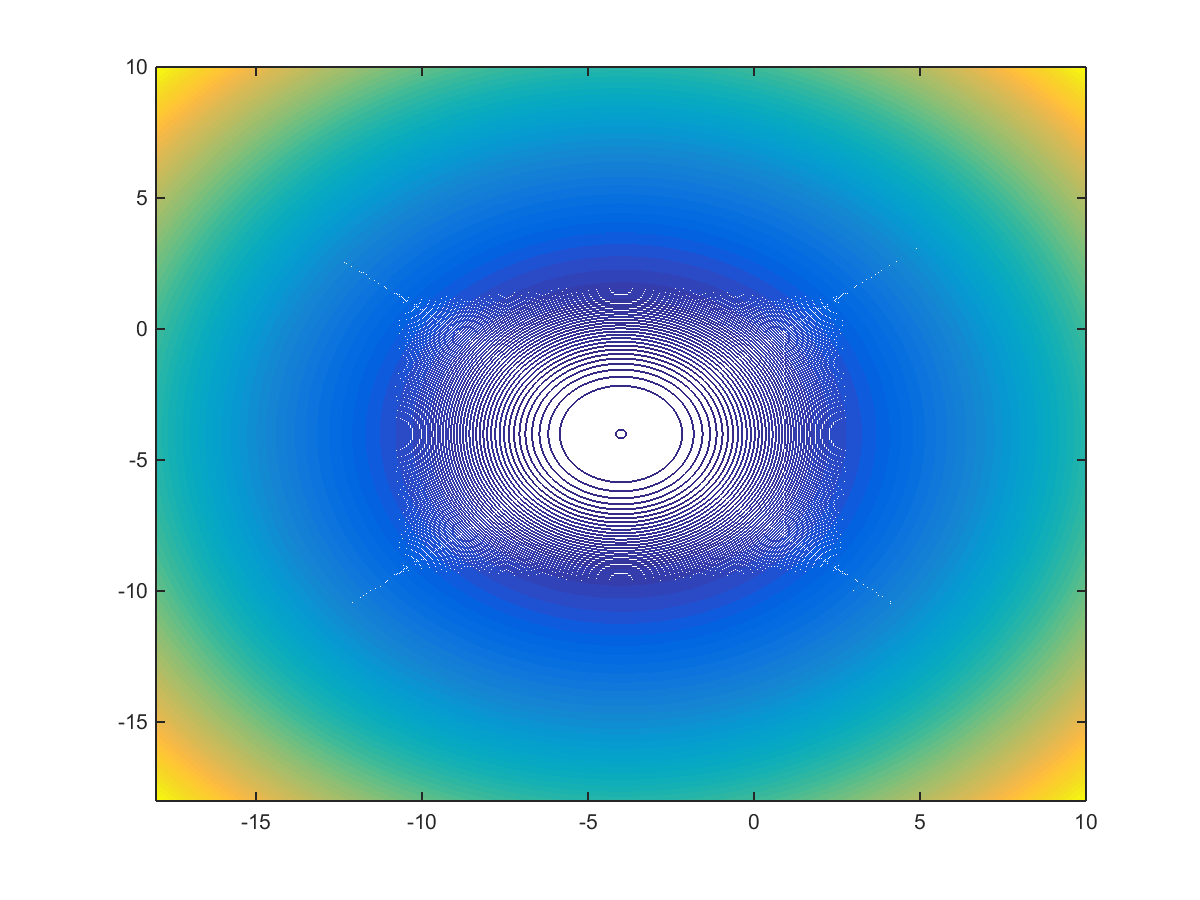
\includegraphics[width=0.5\textwidth]{9688point_contour.png}
 	\caption{Contour of the function ~\ref{eq:main_function} depending on the center of the circle}
 	\label{fig:m96882d}
 \end{figure}
  \begin{figure}[h]
  	\centering
  	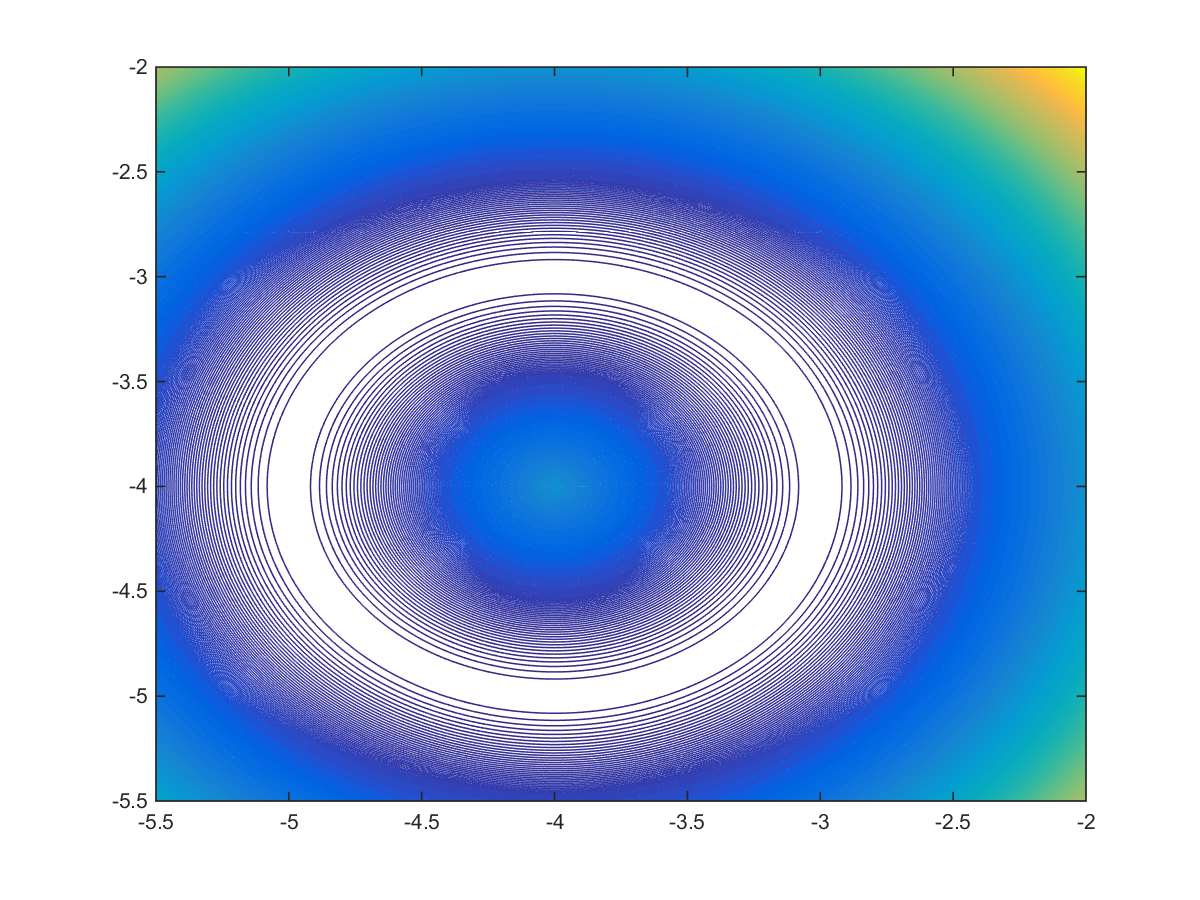
\includegraphics[width=0.5\textwidth]{9688point_contour_close.png}
  	\caption{Closer look at the  contour of the function ~\ref{eq:main_function} depending on the center of the circle}
  	\label{fig:m96882dc}
  \end{figure}
 
 \clearpage
\subsection{}
\subsubsection{Is function \ref{eq:main_function} a differentiable one?}
Yes
\subsubsection{Does function \ref{eq:main_function} has one or many local minimum?}
\paragraph{}
In perfect state function ~\ref{eq:main_function} has a local minimum if we place our circle perfectly, so all points are on the border of this circle.
\paragraph{}
Number of the minimums depends on $ \mathbf{A}, m,  \mathbf{x}$ and $r$. 
As it can be seen in the section  ~\ref{section_1}, for only one given point, there are infinitely many local minimums, because we can place one point on the border of circle infinitely many ways.
In the section  ~\ref{section_2} we had two points, distance between those points was smaller than $ d = 2r $, so there are two ways to place out circle, which gives us two local minimums.
What about minimum number of points needed to define a circle - three? For given three points there will be only one local minimum.
\section{}
\paragraph{Gauss-Newton}
Convergence of Gauss-Newton algorithm is not guaranteed, not even local, as in Newton method. 
\cite{Gauss–Newton algorithm}
\paragraph{Levenberg–Marquardt}
On one hand LM in many cases can find solution even if input parameters are far from the final minimum, on the other hand for reasonable input data LM need more iterations, compared to GN. LM finds only a local minimum. \cite{Levenberg–Marquardt algorithm}
\paragraph{Conclusion} 
For different data we always should apply different algorithm. Why sometimes for speed we should use Leveberg-Marqurdt algorithm, our result depends significantly on the initial data. 

\clearpage
\section{}
 \begin{itemize}
 	\item $m = 1$ 
 	\item $ \mathbf{A} = [0 \: 0] $
 	\item $ X_0 = [1 \: 1] $
 	\item $ r_0 = 2	$
 	\item $ X_1 = [-1 \: -1] $
 	\item $ r_1 = 2	$
 \end{itemize}
  \begin{figure}[h]
  	\centering
  	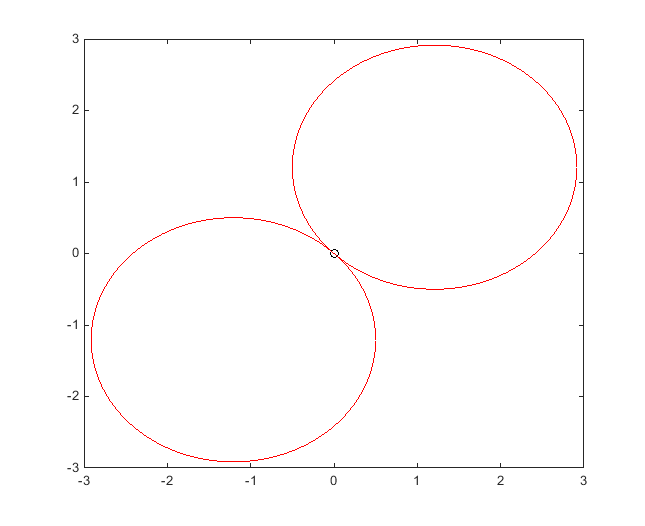
\includegraphics[width=0.4\textwidth]{1point_diff.png}
  	\caption{Result of NL fitting depending on given circle position}
  	\label{fig:1point_diff}
  \end{figure}
  \paragraph{}  For one point ~\ref{fig:1point_diff} there are  infinitely many ways to fit a circle perfectly, there is no way to say which approximation is the right one. For two points, considering that distance between those two points is less than diameter of the circle, there are two possibilities to fit the circle perfectly. And still, for given information (without additional conditions) we can't tell, which approximation is better. 
  \paragraph{} Lets say we have a set of points  $ \mathbf{A} $ that can be almost perfectly be fitted by circle with small noise. Than if we place a first-iteration circle inside a future approximation ~\ref{fig:example1}, it will convergent more faster, than if we would place it outside (so the center of a circle is outside of approximation as well)~\ref{fig:example2} If we would place a first-iteration circle outside, but with center inside, that would be as fast as if we would place a first-iteration circle inside a future approximation.
  \paragraph{} Example above shows us, that if we put all out points  $ \mathbf{A} $  in the quarter of out circle in the first iteration, Levenberg–Marquardt could divergent. 	
  \paragraph{} Another example for given data $ \mathbf{A} $ is to choose one point from set $ \mathbf{A} $ as the center of a circle and set the radius close to the radius of final approximation ~\ref{fig:example3}. In this example Gauss-Newton algorithm will divergent. 
  
  
   \begin{figure}[h]
   	\centering
   	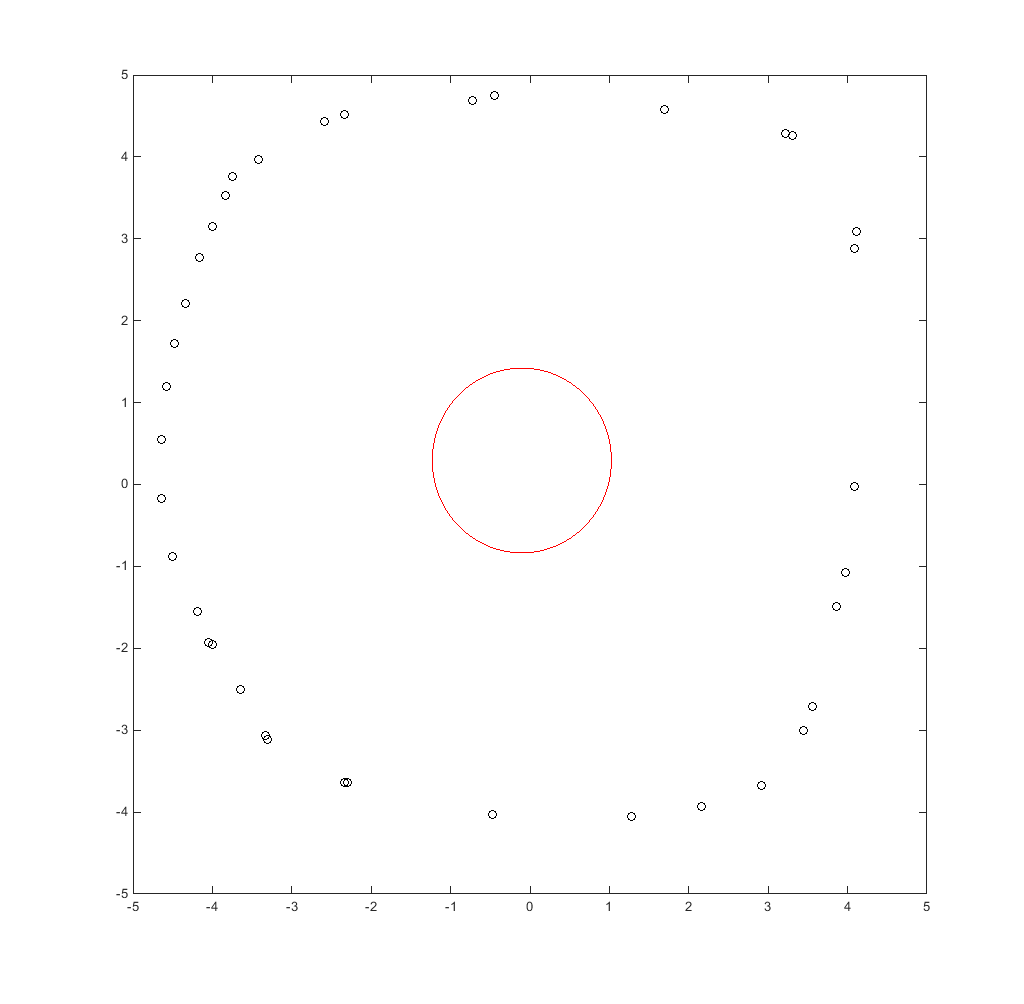
\includegraphics[width=0.35\textwidth]{example1.eps}
   	\caption{Example of input data. Center and borders are inside.}
   	\label{fig:example1}
   \end{figure}
     \begin{figure}[h]
     	\centering
     	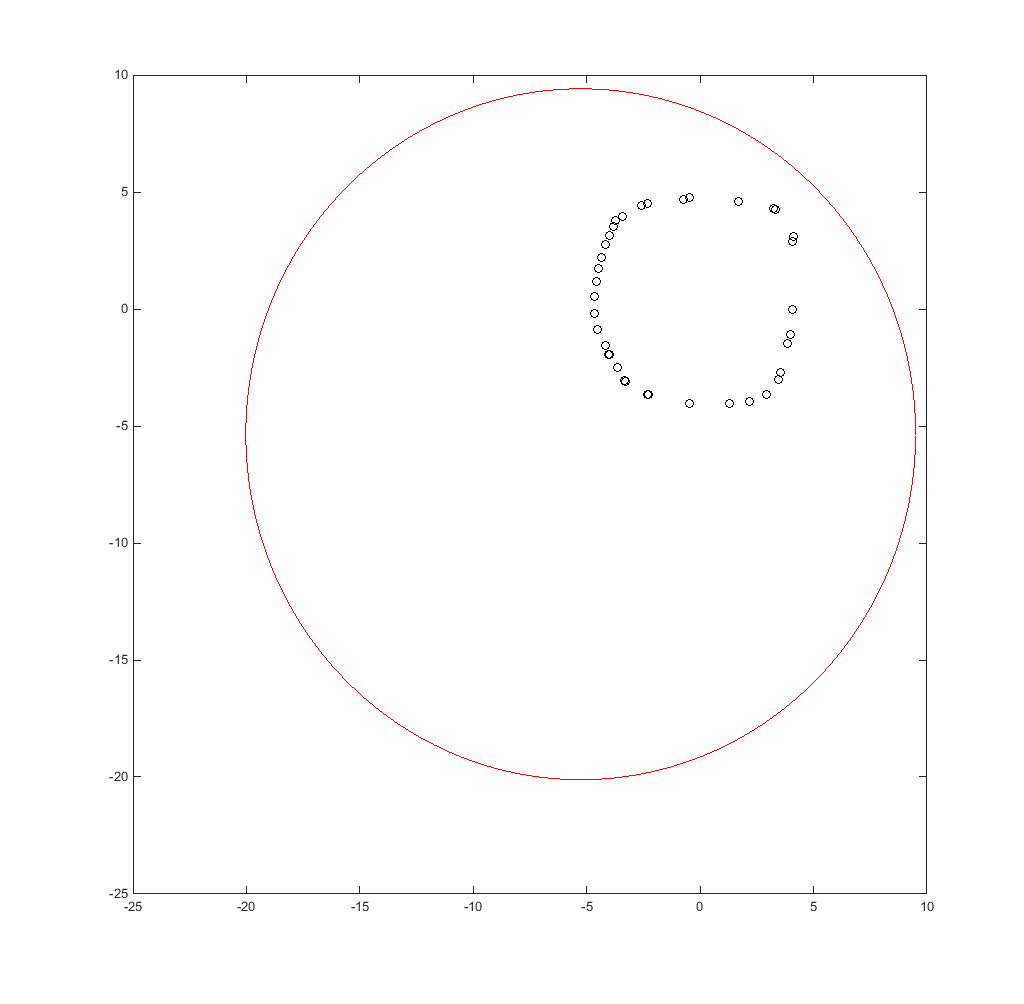
\includegraphics[width=0.35\textwidth]{example2.eps}
     	\caption{Example of input data. Center and borders are outside.}
     	\label{fig:example2}
     \end{figure}
          \begin{figure}[h]
          	\centering
          	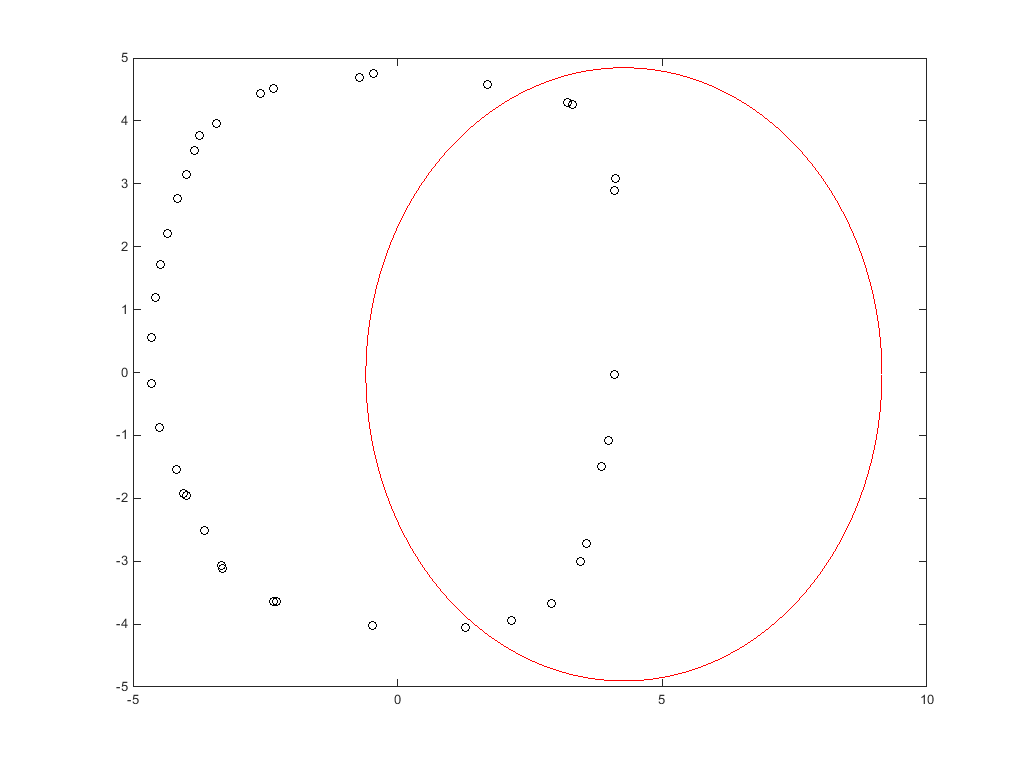
\includegraphics[width=0.35\textwidth]{example3.eps}
          	\caption{Example of input data. Center is one of the points from   $ \mathbf{A} $.}
          	\label{fig:example3}
          \end{figure}
   
  
\newpage
\begin{thebibliography}{1}
	\bibitem{Gauss–Newton algorithm}
	Gauss – Newton algorithm
	\url{http://en.wikipedia.org/wiki/Gauss%E2%80%93Newton_algorithm}
		

	\bibitem{Levenberg–Marquardt algorithm}
	Levenberg – Marquardt algorithm
	\url{http://en.wikipedia.org/wiki/Levenberg%E2%80%93Marquardt_algorithm}
	
\end{thebibliography}
 

\end{document}          
